\providecommand{\main}{..}		% Override relative path to the main file (already set in main file)
\documentclass[../InterneDSLs.tex]{subfiles}
\begin{document}

\section{Hauptteil}
Für die Verarbeitung der \ac{EBNF}-Grammatiken wird ANTLR4 verwendet, der Parser und Lexer für Java generieren kann.

\subsection{Parser}
Als Parser-Generator wurde ANTLR4 verwendet, der Parser zu einer EBNF-Grammatik in Java generieren kann. Dafür verwendet ANTLR aber eine unübliche Syntax, die sich an einer alten EBNF-Variante orientiert.

Der von ANTLR generierte Parser wird von einem Listener erweitert, der aus den EBNF-Konstrukten (die praktisch Strings entprechen) einen Baum aus eigenen Klassen generiert. Dadurch wird eine Typ-Sicherheit hergestellt, die durch die EBNF selbst nicht gegeben ist.

\subsection{Abbildung von EBNF auf Interfaces}
Zuerst wird die in EBNF geschriebene Grammatik in einen Baum aus Java-Objekten transformiert. Dadurch wird eine Typ-Sicherheit hergestellt und Methoden implementiert werden, die das Traversieren des Baumes vereinfachen. Abbildung~\ref{FIG:TypesBNF} zeigt die Typen und ihre Beziehungen untereinander.

\begin{figure}[ht]
\centering
\includegraphics[width=\linewidth]{\main/10_Pictures/BNF-Types}
\caption{Typen des BNF-Baumes}
\label{FIG:TypesBNF}
\end{figure}

\subsubsection{Parse-Tree}


\subsubsection{Abbildung von Kanten auf Interfaces}
Um die Interfaces generieren zu können, müssen die Kanten der Graphen zwischen den Scopes, auf Interfaces abgebildet werden.

Im einfachsten Fall von einer Kante, die nur einen Sequenz-Knoten beinhaltet, kann man den ein Interface mit dem Namen des Knotens und dem nächsten Scope als Rückgabewert erstellen. Grafik~\ref{FIG:SequenceNode} zeigt, wie eine Abbildung aussehen kann.
\begin{figure}[ht]
\centering
  \begin{subfigure}[b]{0.49\textwidth}
    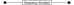
\includegraphics[width=.95\linewidth]{\main/10_Pictures/Nodes_one-element}
    \caption{Diagramm eines Sequenz-Knoten}
    \label{FIG:DiagramSequenceNode}
  \end{subfigure}
  \begin{subfigure}[b]{0.49\textwidth}
    \lstinputlisting[language=Java]{Scope_one-element.java}
    \caption{Java-Interface aus einem Sequenz-Knoten}
    \label{FIG:JInterfaceSequenceNode}
  \end{subfigure}
  \caption{Diagramm und Interface eines Sequenz-Knotens}
  \label{FIG:SequenceNode}
\end{figure}

Falls eine Kante mehrere Alternativen enthält, können die alternativen je als eine Methode in einem Interface implementiert werden, die jeweils den folgenden Scope zurück geben (siehe Abbildung~\ref{FIG:AlternativeNode}).
\begin{figure}[ht]
\centering
  \begin{subfigure}[b]{0.49\textwidth}
    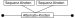
\includegraphics[width=.95\linewidth]{\main/10_Pictures/Nodes_alternative}
    \caption{Diagramm eines Sequenz-Knoten}
    \label{FIG:DiagramAlternativeNode}
  \end{subfigure}
  \begin{subfigure}[b]{0.49\textwidth}
    \lstinputlisting[language=Java]{Scope_alternative.java}
    \caption{Java-Interface aus einem Sequenz-Knoten}
    \label{FIG:JInterfaceAlternativeNode}
  \end{subfigure}
  \caption{Diagramm und Interface eines Sequenz-Knotens}
  \label{FIG:AlternativeNode}
\end{figure}


\subsection{Sprachdesign}


\subsubsection{Einschränkungen}


\end{document}
